\model{Linked Lists}

Linked structures ``chain'' elements using references.
Each element of the list is called a \textit{node}.

\vspace{1ex}
\begin{minipage}{0.40\linewidth}
\begin{javalst}
    public class Node
    {
        private int value;
        private Node next;
        ...
    }
\end{javalst}
\end{minipage}
\hfill
\begin{minipage}{0.58\linewidth}
\begin{javalst}
    Node node3 = new Node(14, null);
    Node node2 = new Node(6, node3);
    Node numbers = new Node(22, node2);
\end{javalst}
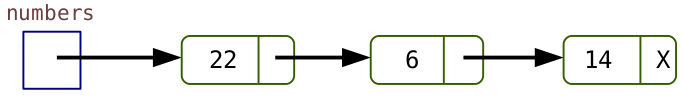
\includegraphics[scale=0.35]{figs/list1.png}
\end{minipage}
\vspace{1em}

This organization allows fast insertions/deletions near the beginning. For example, to add 8:

\vspace{1ex}
\begin{minipage}{0.48\linewidth}
\begin{javalst}
    Node temp = new Node(8, numbers);



    numbers = temp;
\end{javalst}
\end{minipage}
\hfill
\begin{minipage}{0.50\linewidth}
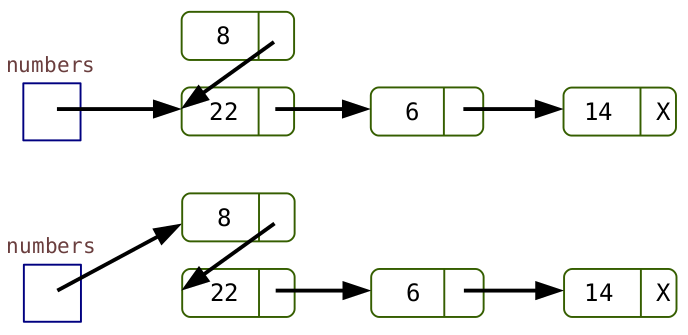
\includegraphics[scale=0.35]{figs/list2.png}
\end{minipage}
\vspace{1em}

Instead of working with nodes directly, we can design a wrapper class to handle list logic:

\vspace{1ex}
\begin{minipage}{0.40\linewidth}
\begin{javalst}
    public class MyList
    {
        private int size;
        private Node head;
        ...
    }
\end{javalst}
\end{minipage}
\hfill
\begin{minipage}{0.58\linewidth}
\begin{javalst}
    MyList numbers = new MyList();
    numbers.addAtStart(14);
    numbers.addAtStart(6);
    numbers.addAtStart(22);
\end{javalst}
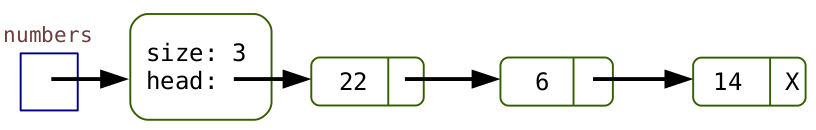
\includegraphics[scale=0.35]{figs/list3.png}
\end{minipage}
\vspace{1ex}


\quest{12 min}


\Q How many operations are required to add 14 \textit{at the start} of an empty list?

\begin{answer}
3 operations: 1 to create the new element, another to copy the reference to the current front, and a third to move the head reference to the new element.
\end{answer}


\Q How many operations are required to add 22 after 14 and 6 have been added?

\begin{answer}
Still just 3: same as the first insert. No shifting is required.
\end{answer}


\Q Using this model, how many operations are required to add another element \textit{at the end} of the current list?

\begin{answer}
5 operations: 3 to find where the new element goes (by following the references to the end of the list), one to create the new node, and one to change the reference of the previous last element.
\end{answer}


\Q How much memory is needed to store each element in the \java{LinkedList}?
How does that amount compare with using an \java{ArrayList}?

\begin{answer}[5em]
The amount needed to store a single element of that type, plus room to store the \java{next} reference of each element.
In this case, 16 bytes for the \java{Integer} object, and 8 bytes for the \java{next} reference.
Arrays require 8 bytes for each reference plus 16 bytes for each object, so it's a wash.
\end{answer}


\Q Discuss why \java{LinkedList} is a poor choice of \java{List} in the program below.

\begin{javabox}
import java.util.LinkedList;
import java.util.List;

public class LinksAreBad
{
    public static void main(String[] args)
    {
        LinkedList<String> linkedList = new LinkedList<>();

        System.out.println("LinkedList: ");
        addAndGet(linkedList);
        System.out.println("Done!");
    }

    public static void addAndGet(List<String> list)
    {
        for (int i = 0; i < 1000000; i++)
        {
            list.add("A");  // add at the end
        }

        for (int i = 0; i < 1000000; i++)
        {
            list.get(list.size() / 2);  // get the middle element
        }
    }
}
\end{javabox}
